%! TeX encoding = UTF-8 unicode
%%%%%%%%%%%%%%%%%%%%%%%%%%%%%%%

\documentclass[10pt,aps,prb,amsmath,amssymb,twocolumn,letterpaper,nobalancelastpage,final,citeautoscript,floatfix,raggedbottom,superscriptaddress]{revtex4-1}

%%%%%%%%%%%%%%%
% MY SETTINGS
%%%%%%%%%%%%%%%v
\usepackage[usenames,dvipsnames]{color}
\usepackage{graphicx}
\usepackage{microtype}
\usepackage[bookmarks=false,colorlinks]{hyperref}
\usepackage{xfrac}
\hypersetup{
    linkcolor=RubineRed,          % color of internal links
    citecolor=ForestGreen,        % color of links to bibliography
    filecolor=Mulberry,      % color of file links
    urlcolor=RoyalBlue           % color of external links
}
\usepackage{natbib}
\usepackage{listings}
%additional commands
\newcommand{\textapprox}{\raisebox{0.5ex}{\texttildelow}}
\newcommand{\gvs}{GaV$_4$S$_8$}
\newcommand{\gvse}{GaV$_4$Se$_8$}
\newcommand{\gms}{GaMo$_4$S$_8$}
\newcommand{\gmse}{GaMo$_4$Se$_8$}
\newcommand{\gns}{GaNb$_4$S$_8$}
\newcommand{\gnse}{GaNb$_4$Se$_8$}
\newcommand{\gts}{GaTa$_4$S$_8$}
\newcommand{\gtse}{GaTa$_4$Se$_8$}

\newcommand{\dpg}[1]{\textcolor{red}{#1}}


%%%%%%%%%%%%%
% MAIN TEXT
%%%%%%%%%%%%%

\begin{document}

\title{Analysis of alloy steel composition-property \\ relationship using machine learning}

\author{Raymond Wang}
  \affiliation{Department of Materials Science and Engineering, Northwestern University, Evanston, Illinois  60208, USA}

  
%%%%%%%%%%%%%
% ABSTRACT
%%%%%%%%%%%%%

\begin{abstract}
This challenge project scrapes digital alloy steel data from online resources and converts them into machine-readable format. Data analysis using correlation heatmap shows degree of correlation within alloy steel composition and properties. Several strongly correlated quantities (e.g. hardness and tensile strength) are identified. Machine learning algorithm performance on predicting composition-property relationship is benchmarked using grid search. XGBoost outperforms the other methods in the alloy steel case. Further analysis shows predicting thermal conductivity from chemical composition using XGBoost has satisfying accuracy and the model performance can be improved by having more training data. Our findings suggest that machine learning methods could provide more insights of alloy steel composition-property relationship than using human physical intuition or experience.
\end{abstract}

\maketitle

%%%%%%%%%%%%%%%%%%%%%%%%%%%%%%%%%%%%%%
% MOTIVATION
%%%%%%%%%%%%%%%%%%%%%%%%%%%%%%%%%%%%%%

\section{Workflow}

The challenge project mainly consists of five sections, i.e. data acquisition, featurization, human interpretation, machine learning model training, and result analysis. The flowchart and specific outcomes in each step are shown in Figure \ref{fig:flowchart}. The rest of this report will span these five sections into details of implementation and obtained results. Data is available at the author's \href{https://github.com/raymond931118/scraping}{GitHub}, the code can be found in supporting information (SI).

\begin{figure}[h]
  \center
  \vspace{-1mm}
 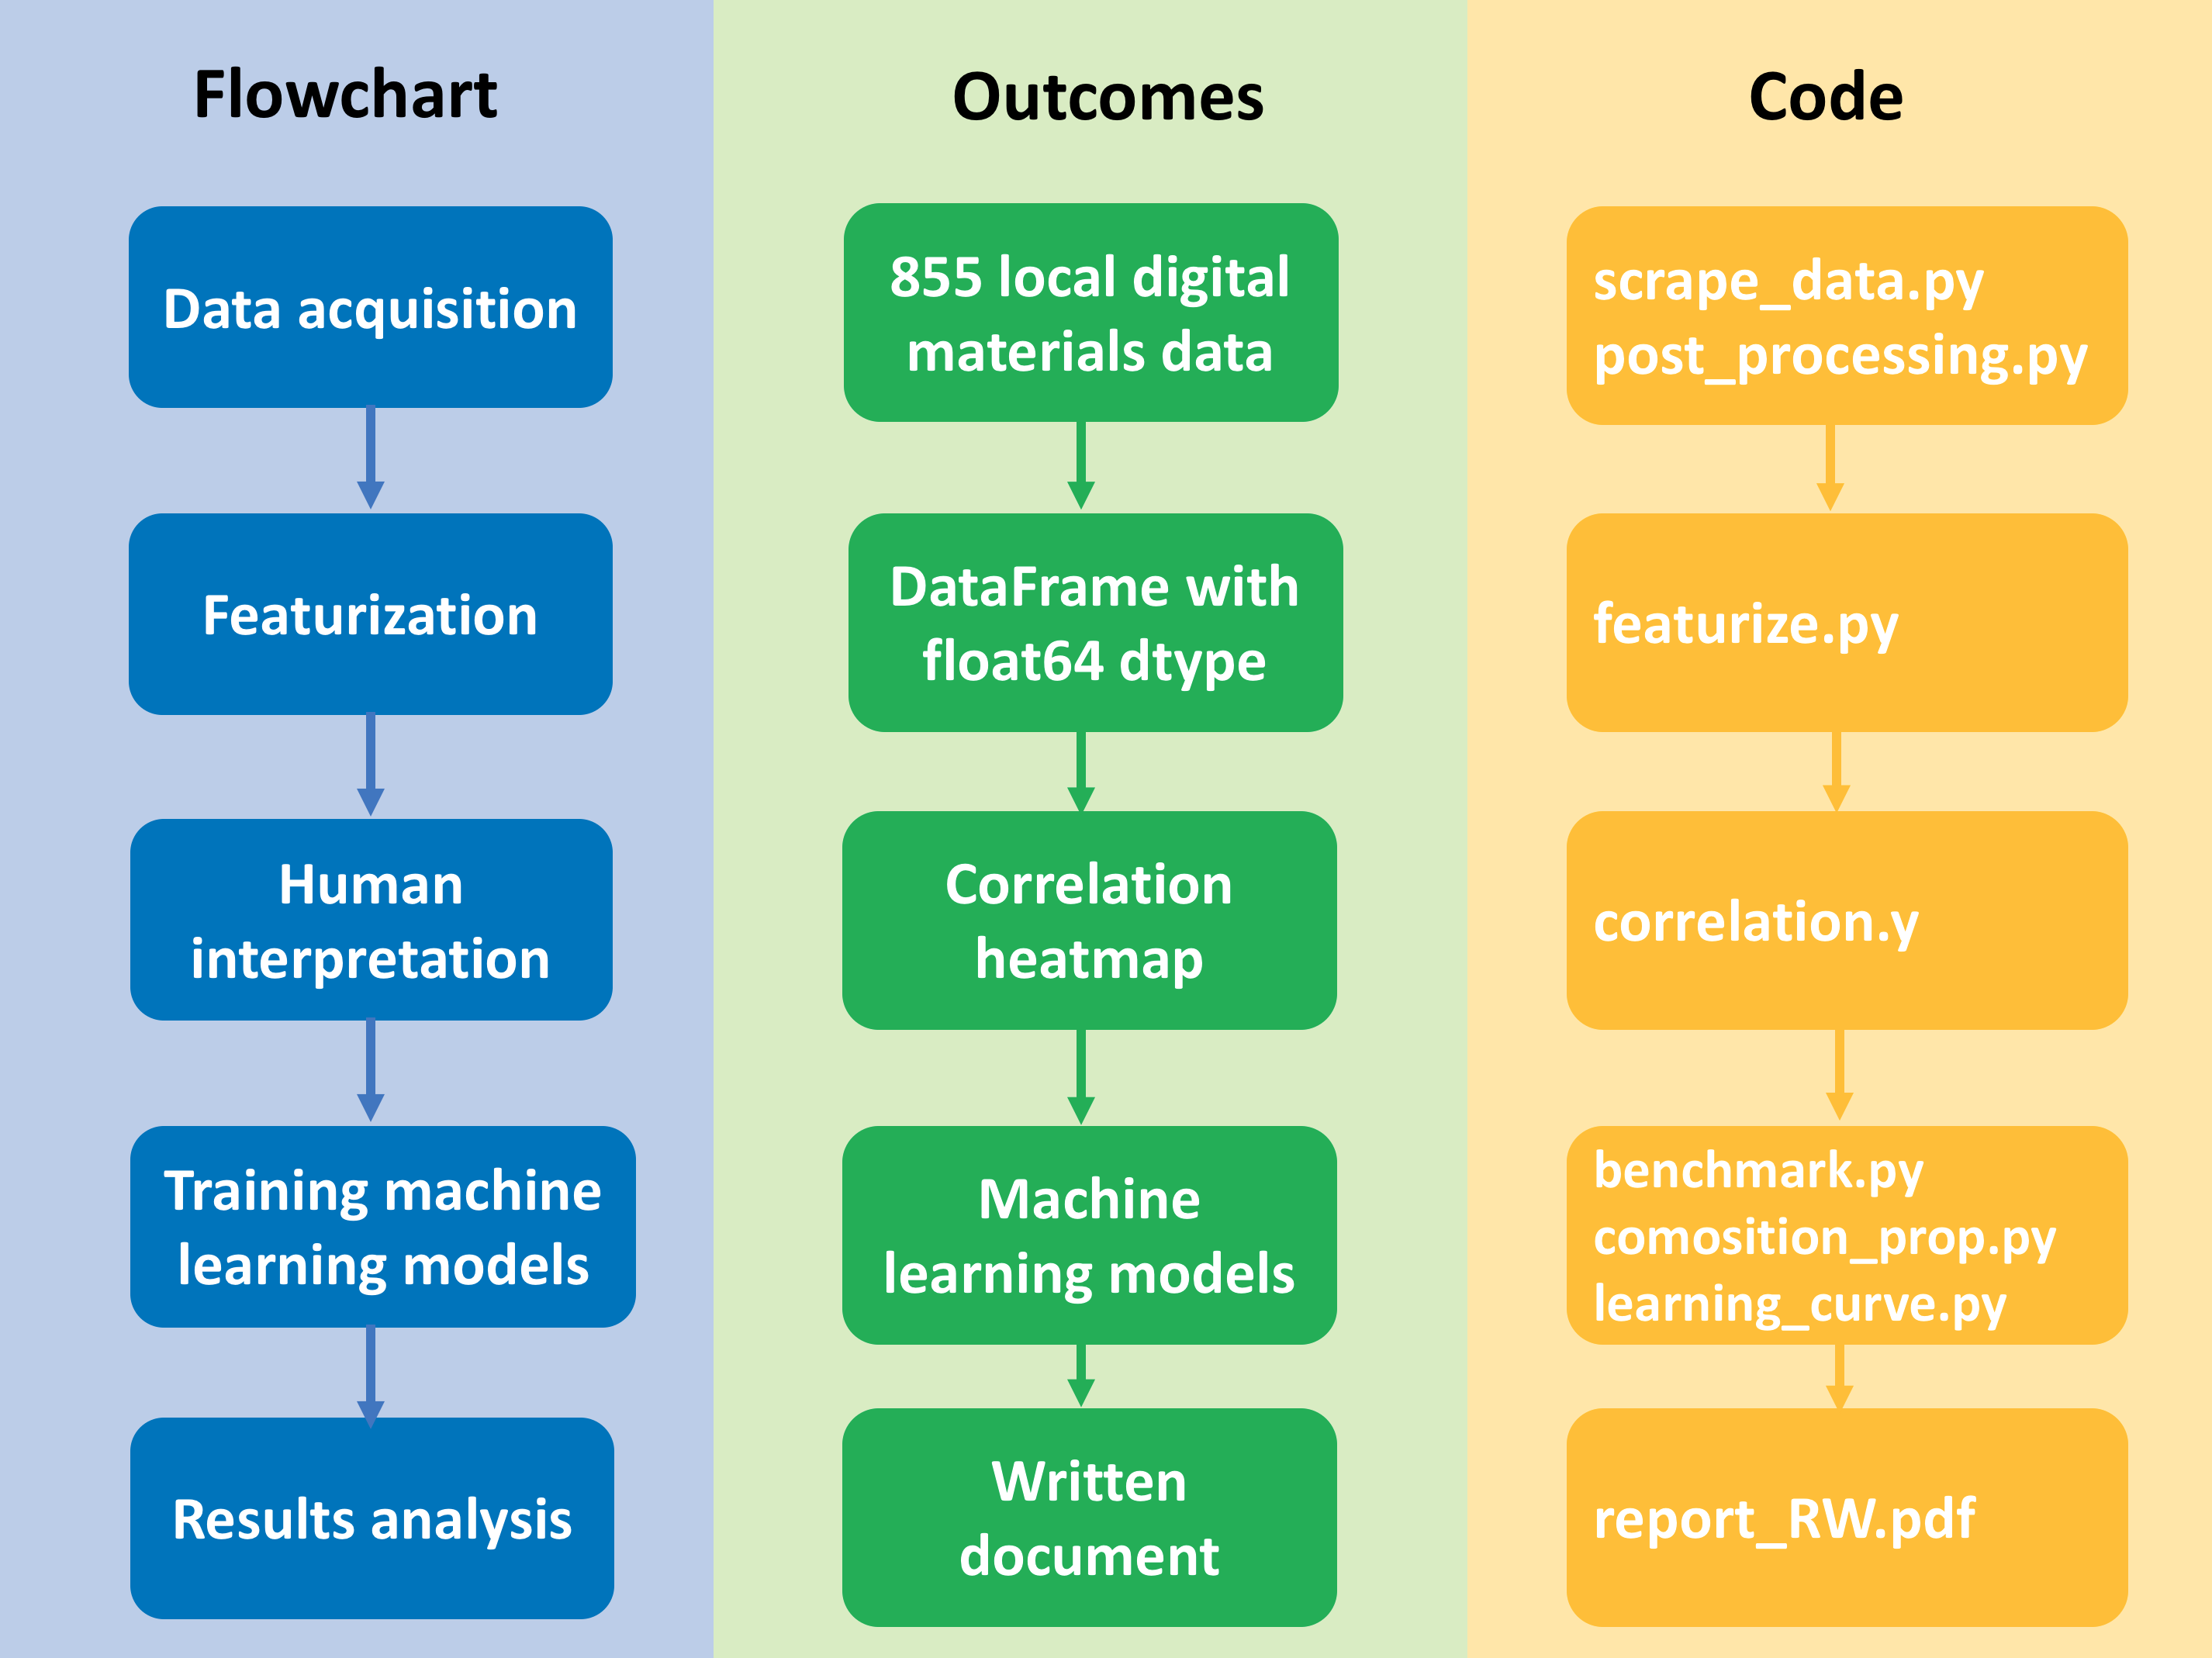
\includegraphics[width=0.95\linewidth]{figures/flowchart.png}
  \caption{Flowchart of the challenge project.}
  \label{fig:flowchart}
\end{figure}




%%%%%%%%%%%%%%%%%%%%%%%%%%%%%%%%%%%%%%
% DATA ACQUISITION
%%%%%%%%%%%%%%%%%%%%%%%%%%%%%%%%%%%%%%
\section{data acquisition}

The challenge project starts from acquiring materials data from online resources. Automated scraping code is developed by the author in Python, which automatically collects materials information that meets the searching criteria and saves to local CSV files. 

Materials data is collected from \href{http://www.matweb.com/index.aspx}{MatWeb}, where alloy steels containing Manganese, Chromium, and Nickel are set as the target materials for scraping. Each entry of material data spans four columns and multiple rows, as shown in Table \ref{tab:web_data}. Data under `English' has different unit from `Metric', this project only processes data with metric unit.

\vspace{-10pt}
\begin{table}[h]
\begin{ruledtabular}
\caption{Format of online resources.\label{tab:web_data}}\centering
\begin{tabular}{llll}
\sffamily Property & \sffamily Metric & \sffamily English &  \sffamily Comments \\
\hline 
Elongation at break & 55\% & 55\% & some comments \\
\hline
$\cdots$ & $\cdots$ & $\cdots$ & $\cdots$
\end{tabular}
\end{ruledtabular}
\end{table}

Physical properties (e.g. bulk modulus, thermal conductivity) in different units, chemical compositions (e.g. weight of Mn, Ni, Cr), and the potentially helpful comments, are saved to local files with unchanged format. Since there is no data-editing involved in this step, the local data is guaranteed to be the same as its online version.

One of the technical challenges during data acquisition is IP-blocking from the web server. MatWeb will block the IP (possibly permanently) once it detects over-access within a short period of time. From the author's experience, one IP address gives access to 100$\sim$200 materials information per day. One of the advantage of the developed code is its high portability. The only two dependencies are \texttt{selenium} and \texttt{pandas} Python packages, which can be installed easily. In order to accelerate the project, the author used six machines with Unix-like systems for development and production. Eventually the program extracted 855 alloy steels that meet the criteria. The code (\hyperlink{scrape}{\texttt{scrape.py}}) is available in SI.

Simple post-processing is performed right after all the data has been saved locally. This step modifies the file names and contents containing non-utf-8 encoding and fixes unwanted line breaks. Relevant code (\hyperlink{pprocess}{\texttt{post\_processing.py}}) is available in SI.

%%%%%%%%%%%%%%%%%%%%%%%%%%%%%%%%%%%%%%
% FEATURIZATION
%%%%%%%%%%%%%%%%%%%%%%%%%%%%%%%%%%%%%%
\section{featurization}

The data collected from the last step is still string-based, e.g. ``97\%'' is interpreted as a sequence of characters instead of a floating point number. Therefore, it is necessary to convert these strings to machine-readable form before any further data analysis.

Since there are multiple materials properties and not all of them are available for each materials, dataset with missing values will be dropped. In order to keep a relatively large number of training set (e.g. several hundred), we only convert and keep physical properties with more than 100 available measured data points. These physical variables are: density, hardness (Vickers), thermal conductivity, specific heat capacity, CTE-linear, electrical resistivity, elongation at break, bulk modulus, modulus of elasticity, shear modulus, poisson's ratio, tensile strength at yield, and tensile strength at ultimate. Ten element types including Fe, Mn, Cr, Ni, Mo, Cu, C, S, Si, P are considered.

Floating point numbers are extracted from string data and converted to \texttt{pandas.DataFrame} format. The converted dataset is shown in Table \ref{tab:featurization}. Non-available data points are converted to \texttt{nan} instead of `N/A'. The `\%' and other units are dropped, only the floating point numbers are extracted. Since data will be standardized before numerical processing, the only thing to make sure is that all data in the same column share the same unit/percentage sign. The code (\hyperlink{featurize}{\texttt{featurize.py}}) is available in SI.

\vspace{-10pt}
\begin{table}[h]
\begin{ruledtabular}
\caption{Format of data after featurization.\label{tab:featurization}}\centering
\begin{tabular}{ccccccc}
\sffamily Fe & \sffamily Mn & \sffamily Cr &  \sffamily $\cdots$ &  \sffamily Hardness &  \sffamily Bulk modulus &  \sffamily $\cdots$ \\
\hline 
97.16 & 0.88 & 0.5 & $\cdots$ & 220 & \texttt{nan} & $\cdots$\\
\hline
95.43 & 0.85 & 0.0 & $\cdots$ & \texttt{nan} & 160 & $\cdots$\\
\hline
$\cdots$ & $\cdots$ & $\cdots$ & $\cdots$ & $\cdots$ & $\cdots$ & $\cdots$
\end{tabular}
\end{ruledtabular}
\end{table}


%%%%%%%%%%%%%%%%%%%%%%%%%%%%%%%%%%%%%%%%%
% DATA ANALYSIS WITH HUMAN INTELLIGENCE
%%%%%%%%%%%%%%%%%%%%%%%%%%%%%%%%%%%%%%%%%
\section{data analysis with human intelligence}

The size of the dataset after featurization is 726$\times$23 (with 726 instances and 23 features). It is impractical for humans (at least for the author) to directly learn patterns from such large amount of data. Based on basic statistical knowledge, the author decides to start from learning correlation patten of these variables. The instances with \texttt{nan} entries are dropped from the dataset, and eventually 254 materials are used to generate the heatmap, as shown in Figure \ref{fig:heatmap}. The code (\hyperlink{correlation}{\texttt{correlation.py}}) can be found in SI.

\begin{figure*}[t]
  \center
 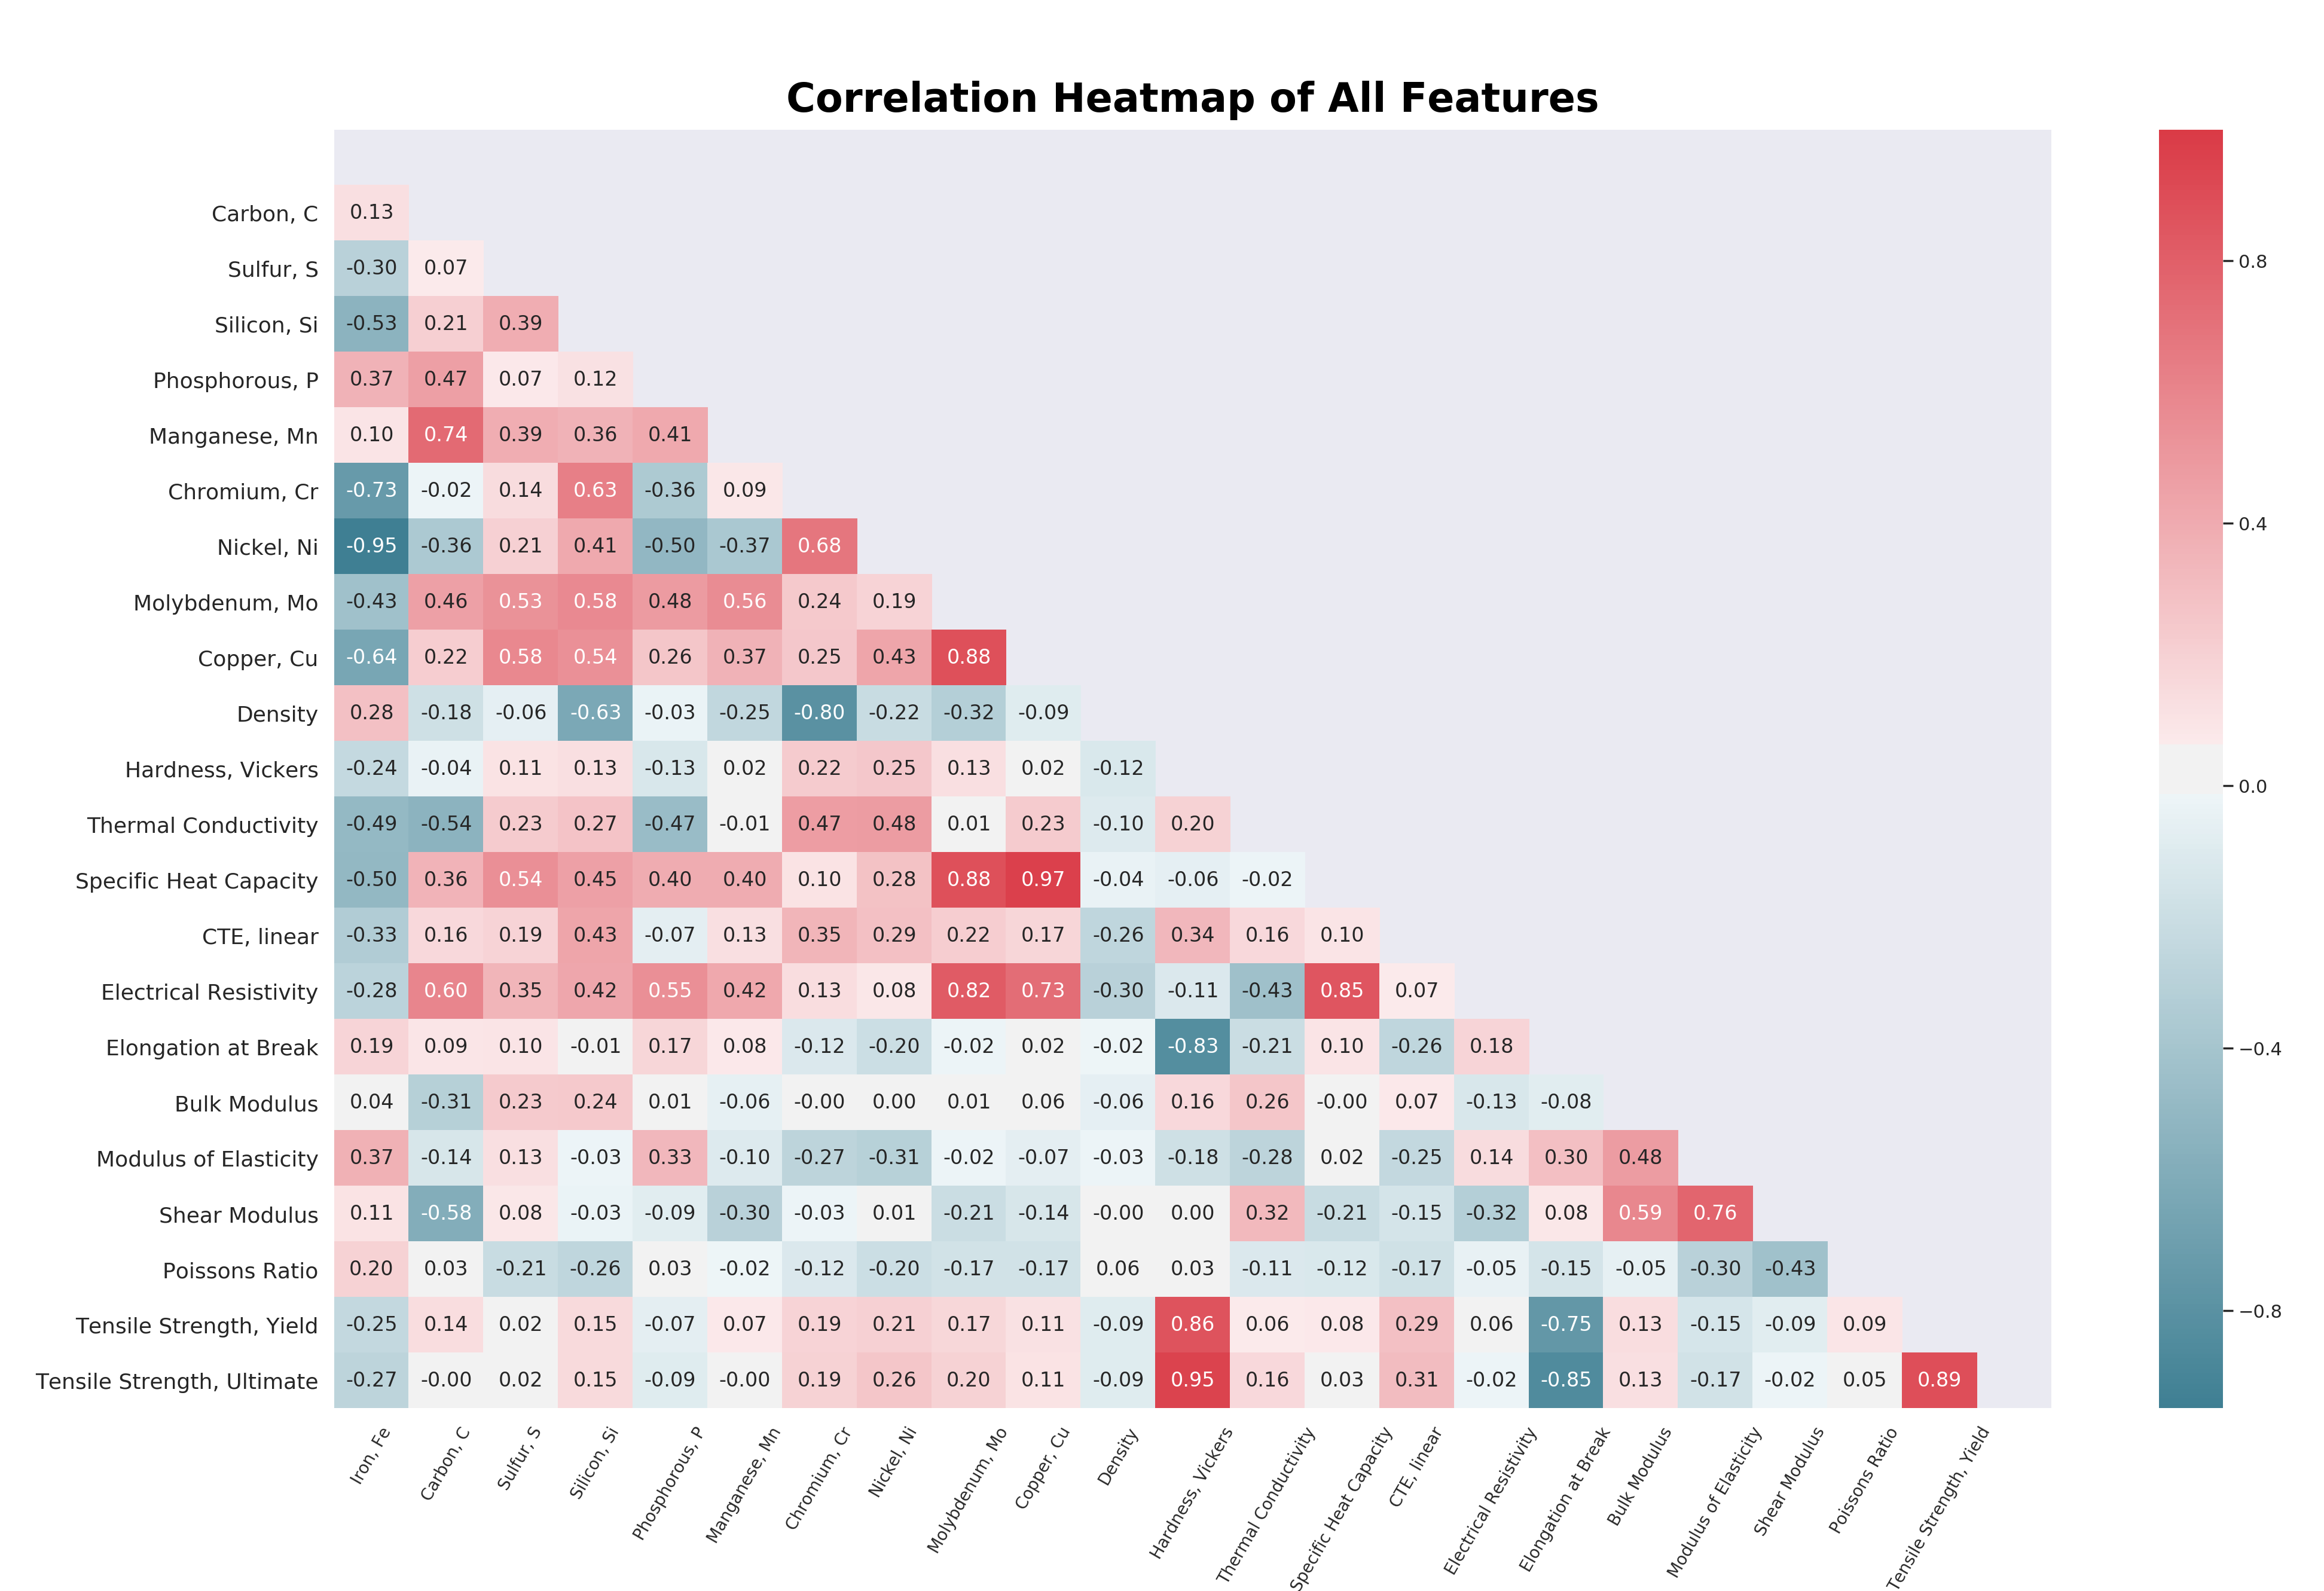
\includegraphics[width=0.85\linewidth]{figures/heatmap_mask.png}
  \caption{Correlation heatmap of chemical composition and physical properties.}
  \label{fig:heatmap}
\end{figure*}

Some of the discoveries from the heatmap include:
\begin{enumerate}
	\item[i.] Carbon increases electrical resistivity but decreases shear modulus
	\item[ii.] Sulfur increases specific heat capacity
	\item[iii.] Phosphorus increases electrical resistivity
	\item[iv.] Chromium decreases density
	\item[v.] Molybdenum and copper strongly increases specific heat capacity and electrical resistivity
	\item[vi.] Nickel increases thermal conductivity
	\item[vii.] Hardness is positively correlated to tensile strength and negatively correlated to elongation at break
	\item[viii.] Electrical resistivity is positively related to specific heat capacity
\end{enumerate}


Some of the findings agree well with the way elements contribute to alloy steel properties as reported online, e.g. carbon decreases ductility of steel, and could lead to a small shear modulus. However, the information from correlation analysis is more qualitative than quantitative. If we want more quantitative descriptions of the materials composition-property relationship, more sophisticated methods are needed. In the next section we discuss alloy steel data analysis using machine learning models.


%%%%%%%%%%%%%%%%%%%%%%%%%%%%%%%%%%%%%%%%%%%%%%
% DATA ANALYSIS WITH ARTIFICIAL INTELLIGENCE
%%%%%%%%%%%%%%%%%%%%%%%%%%%%%%%%%%%%%%%%%%%%%%
\section{data analysis with artificial intelligence}

\subsection{benchmark machine learning algorithm performance on dataset}

The author performs systematic benchmark of different machine learning algorithm performance on various physical property predictions.

Each training takes one physical property as the target, while treats the rest 12 properties plus aforementioned 10 element types as input features. Dataset instances with \texttt{nan} are dropped from the dataset. Numerical data (both X and y) are standardized as implemented in \texttt{StandardScaler} in \texttt{sklearn}.



10 machine learning algorithms are benchmarked here, including:
\begin{enumerate}
	\item Linear Regression	
	\item Least-angle regression with Lasso
	\item Kernel Ridge
	\item Linear SVR
	\item SGD Regression
	\item MLP Regressor
	\item AdaBoost Regression
	\item Random Forest Regression
	\item Gradient Boosting Regression
	\item Extremen Gradient Boosting
\end{enumerate}


The dataset is divided into training (75\%) and testing (25\%) parts. Grid search method is used for hyper-parameter tuning. The set of hyper-parameters are shown in Table \ref{tab:hyperparam} . The optimal setting of the parameters is determined based on 5-fold cross-validation performed on training data only. R2 score is used as error metric. Relevant code (\hyperlink{ml}{\texttt{benchmark.py}})can be found in SI. Results are shown in Figure \ref{fig:benchmark}.


\begin{figure}[h]
  \center
 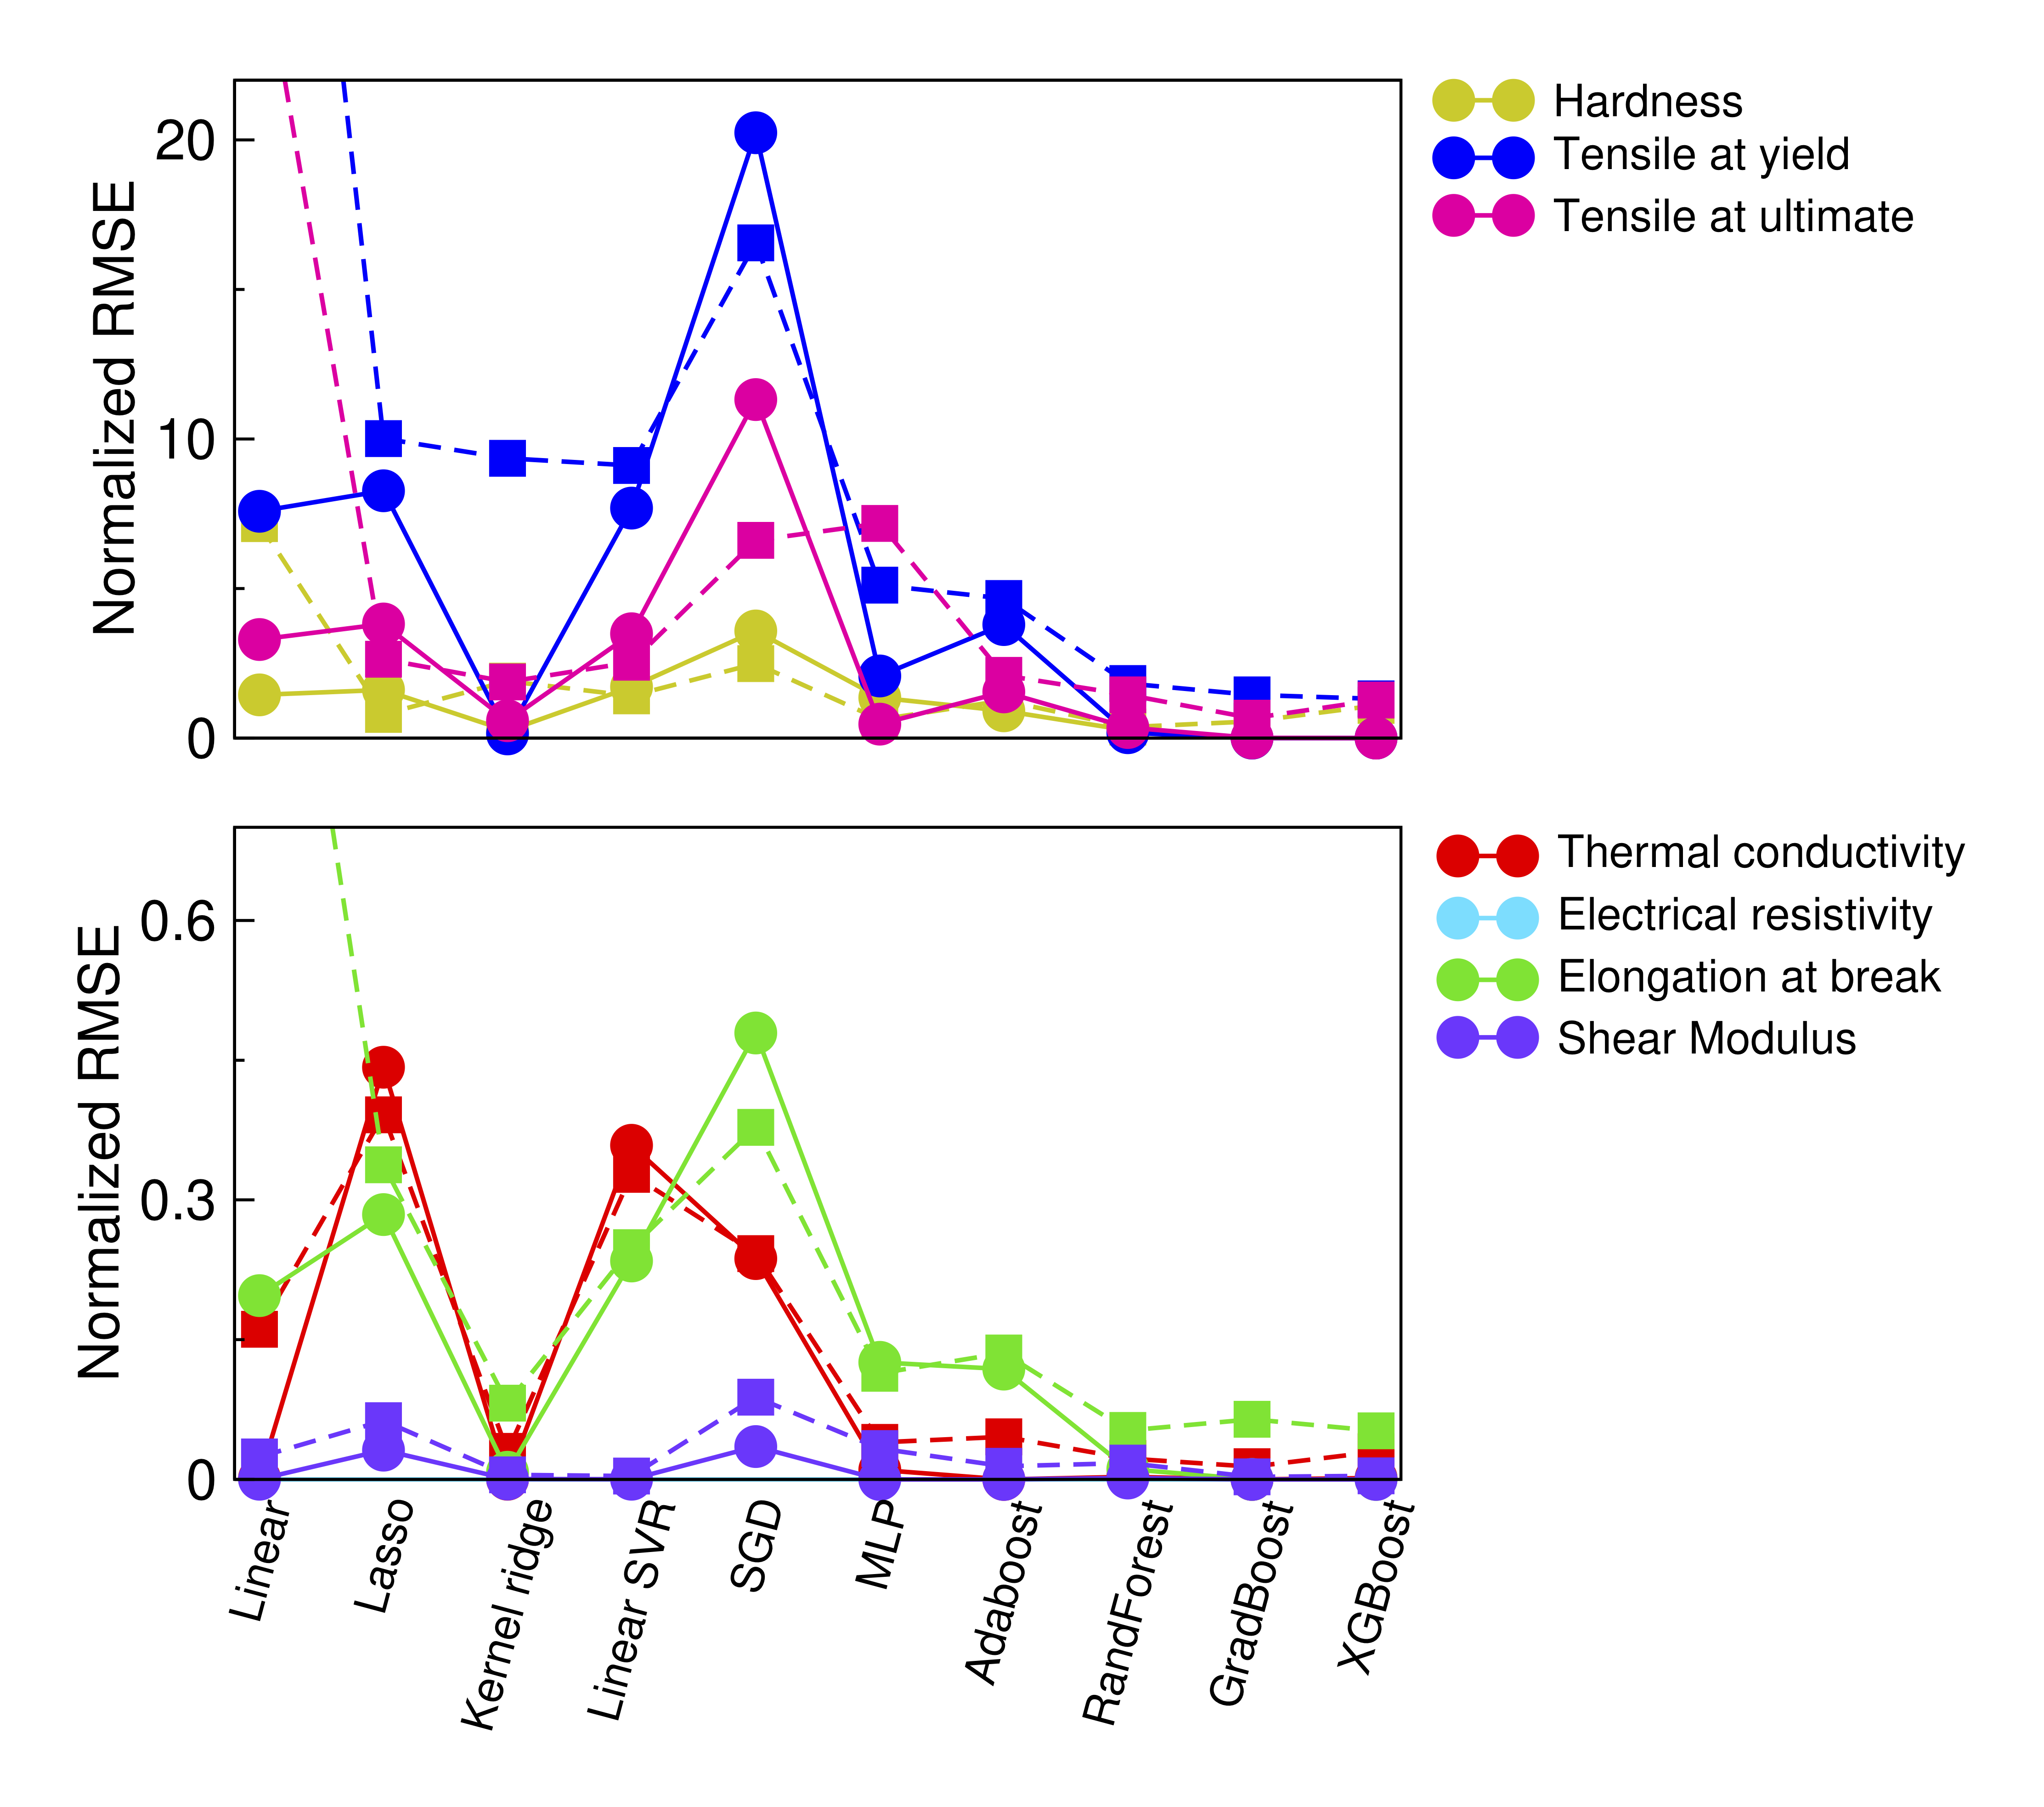
\includegraphics[width=0.95\linewidth]{figures/benchmark.png}
 \vspace{-10pt}
  \caption{Normalized root mean square error (RMSE) of different machine learning algorithms in predicting various physical properties. Training errors are shown in circles and solid lines, test errors are in squares and dashed lines.}
  \label{fig:benchmark}
\end{figure}


The y-axis is the calculated root mean square error (RMSE) value divided by the difference of maximum and minimum value in the target data. This normalization step is essential so as to directly compare the performance of different machine learning algorithms in predicting quantities at various scales. The \texttt{sklearn} built-in performance scores (e.g. R2-score) are not used here.

Interestingly, some trends can be identified across different algorithms as well as physical properties. In general, linear regression, Lasso, linear SVR and SGD algorithms lead to larger variance in normalized RMSE, while the rest have relatively better performance. XGBoost algorithm achieves the best performance among the 10 benchmarked methods.

The physical properties are divided into two panels due to different scales of RMSE. We find it hard to have a good prediction in hardness and tensile strength, but it may not be a coincidence. It is exciting to notice that from the correlation heatmap analysis, it is clear that hardness is strongly and positively correlated to tensile strengths. This may suggest that these quantities are related to some other factors not considered here, such as processing and microscopic structures. And we need to include the other important features in order to build better machine learning models.


\subsection{predict composition-property relationship}

We further investigate machine learning model performance on more challenging problems. In the previous section single property is targeted using both alloy chemical composition and other known physical properties. However in practical situations, sometimes other properties are also unknown (e.g. a new family of alloy steel), would machine learning be able to distill the composition-property relationship to facilitate alloy steel design?

We choose to use Extreme Gradient Boosting (XGBoost) algorithm for further analysis on alloy steel composition-relationship. This time the features only include composition information, i.e. weight percentage of each element. The performance of XGBoost in independently predicting 11 different physical properties is shown in Figure \ref{fig:compo-prop}. R2-score is used as error metric in this case. The implementation of this part is very similar to that in \hyperlink{ml}{\texttt{benchmark.py}} with some small tweaks, the code is not attached in SI but can be found on the author's \href{https://github.com/raymond931118/scraping}{GitHub}.

\begin{figure}[h]
  \center
  \vspace{-1mm}
 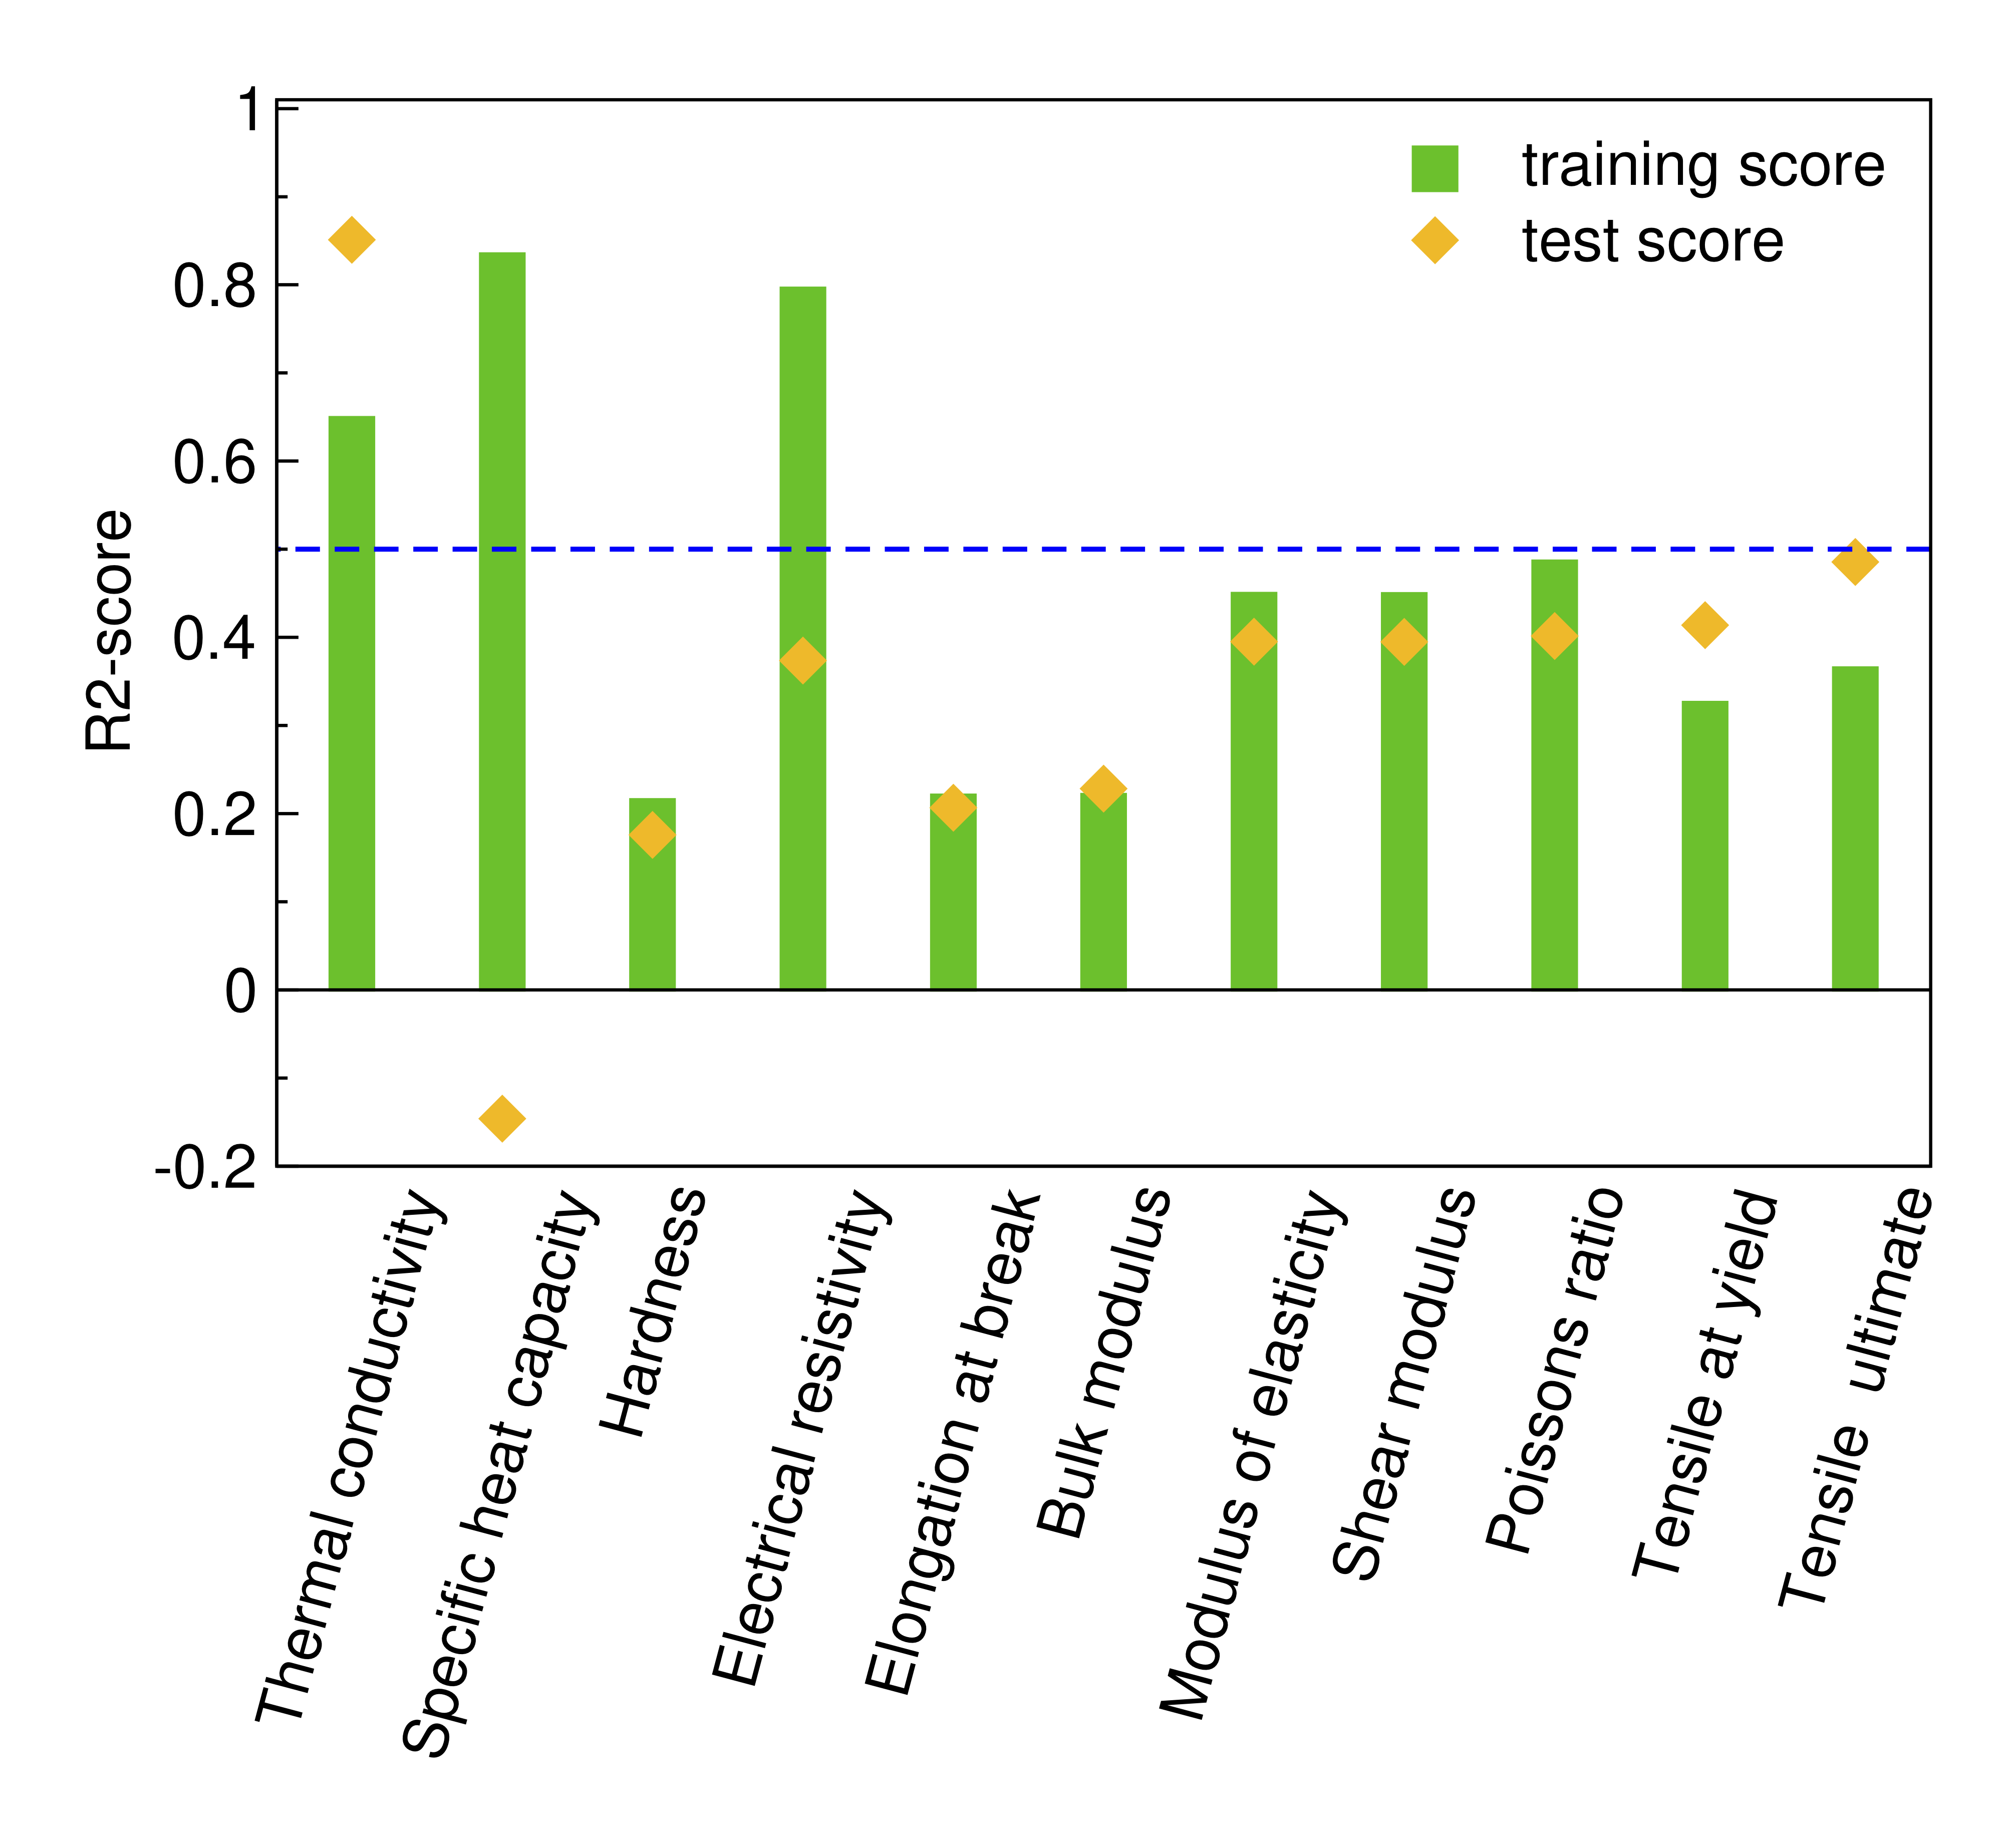
\includegraphics[width=0.95\linewidth]{figures/compo-prop.png}
  \caption{R2-score of XGBoost in predicting 11 physical properties using only chemical composition as features. The dashed line is a border line above which has a `satisfying' score. }
  \label{fig:compo-prop}
\end{figure}

Among the 11 tested properties, 8 of them do not show a strong relationship to composition, both training score and test score are below 0.5. Specific heat capacity and electrical resistivity get a high score in training but score poorly in test. This probably means XGBoost cannot correctly capture the relationship from the training set, but only numerically fit the data. In other words, the model suffers from overfitting. One thing to notice here is that R2-score can be negative, which means the model is even worse than a horizontal line through the mean feature value.

XGBoost performs well in predicting thermal conductivity using composition information, where the test score is even higher than training score. In order to validate our findings, the learning curve of predicting thermal conductivity is shown in Figure \ref{fig:learning_curve}. As the number of training samples increase, cross-validation scores quickly increase and converge to the high training score. This clearly means adding more training samples can further improve the performance of XGBoost model in predicting thermal conductivity.

\begin{figure}[h]
  \center
  \vspace{-1mm}
 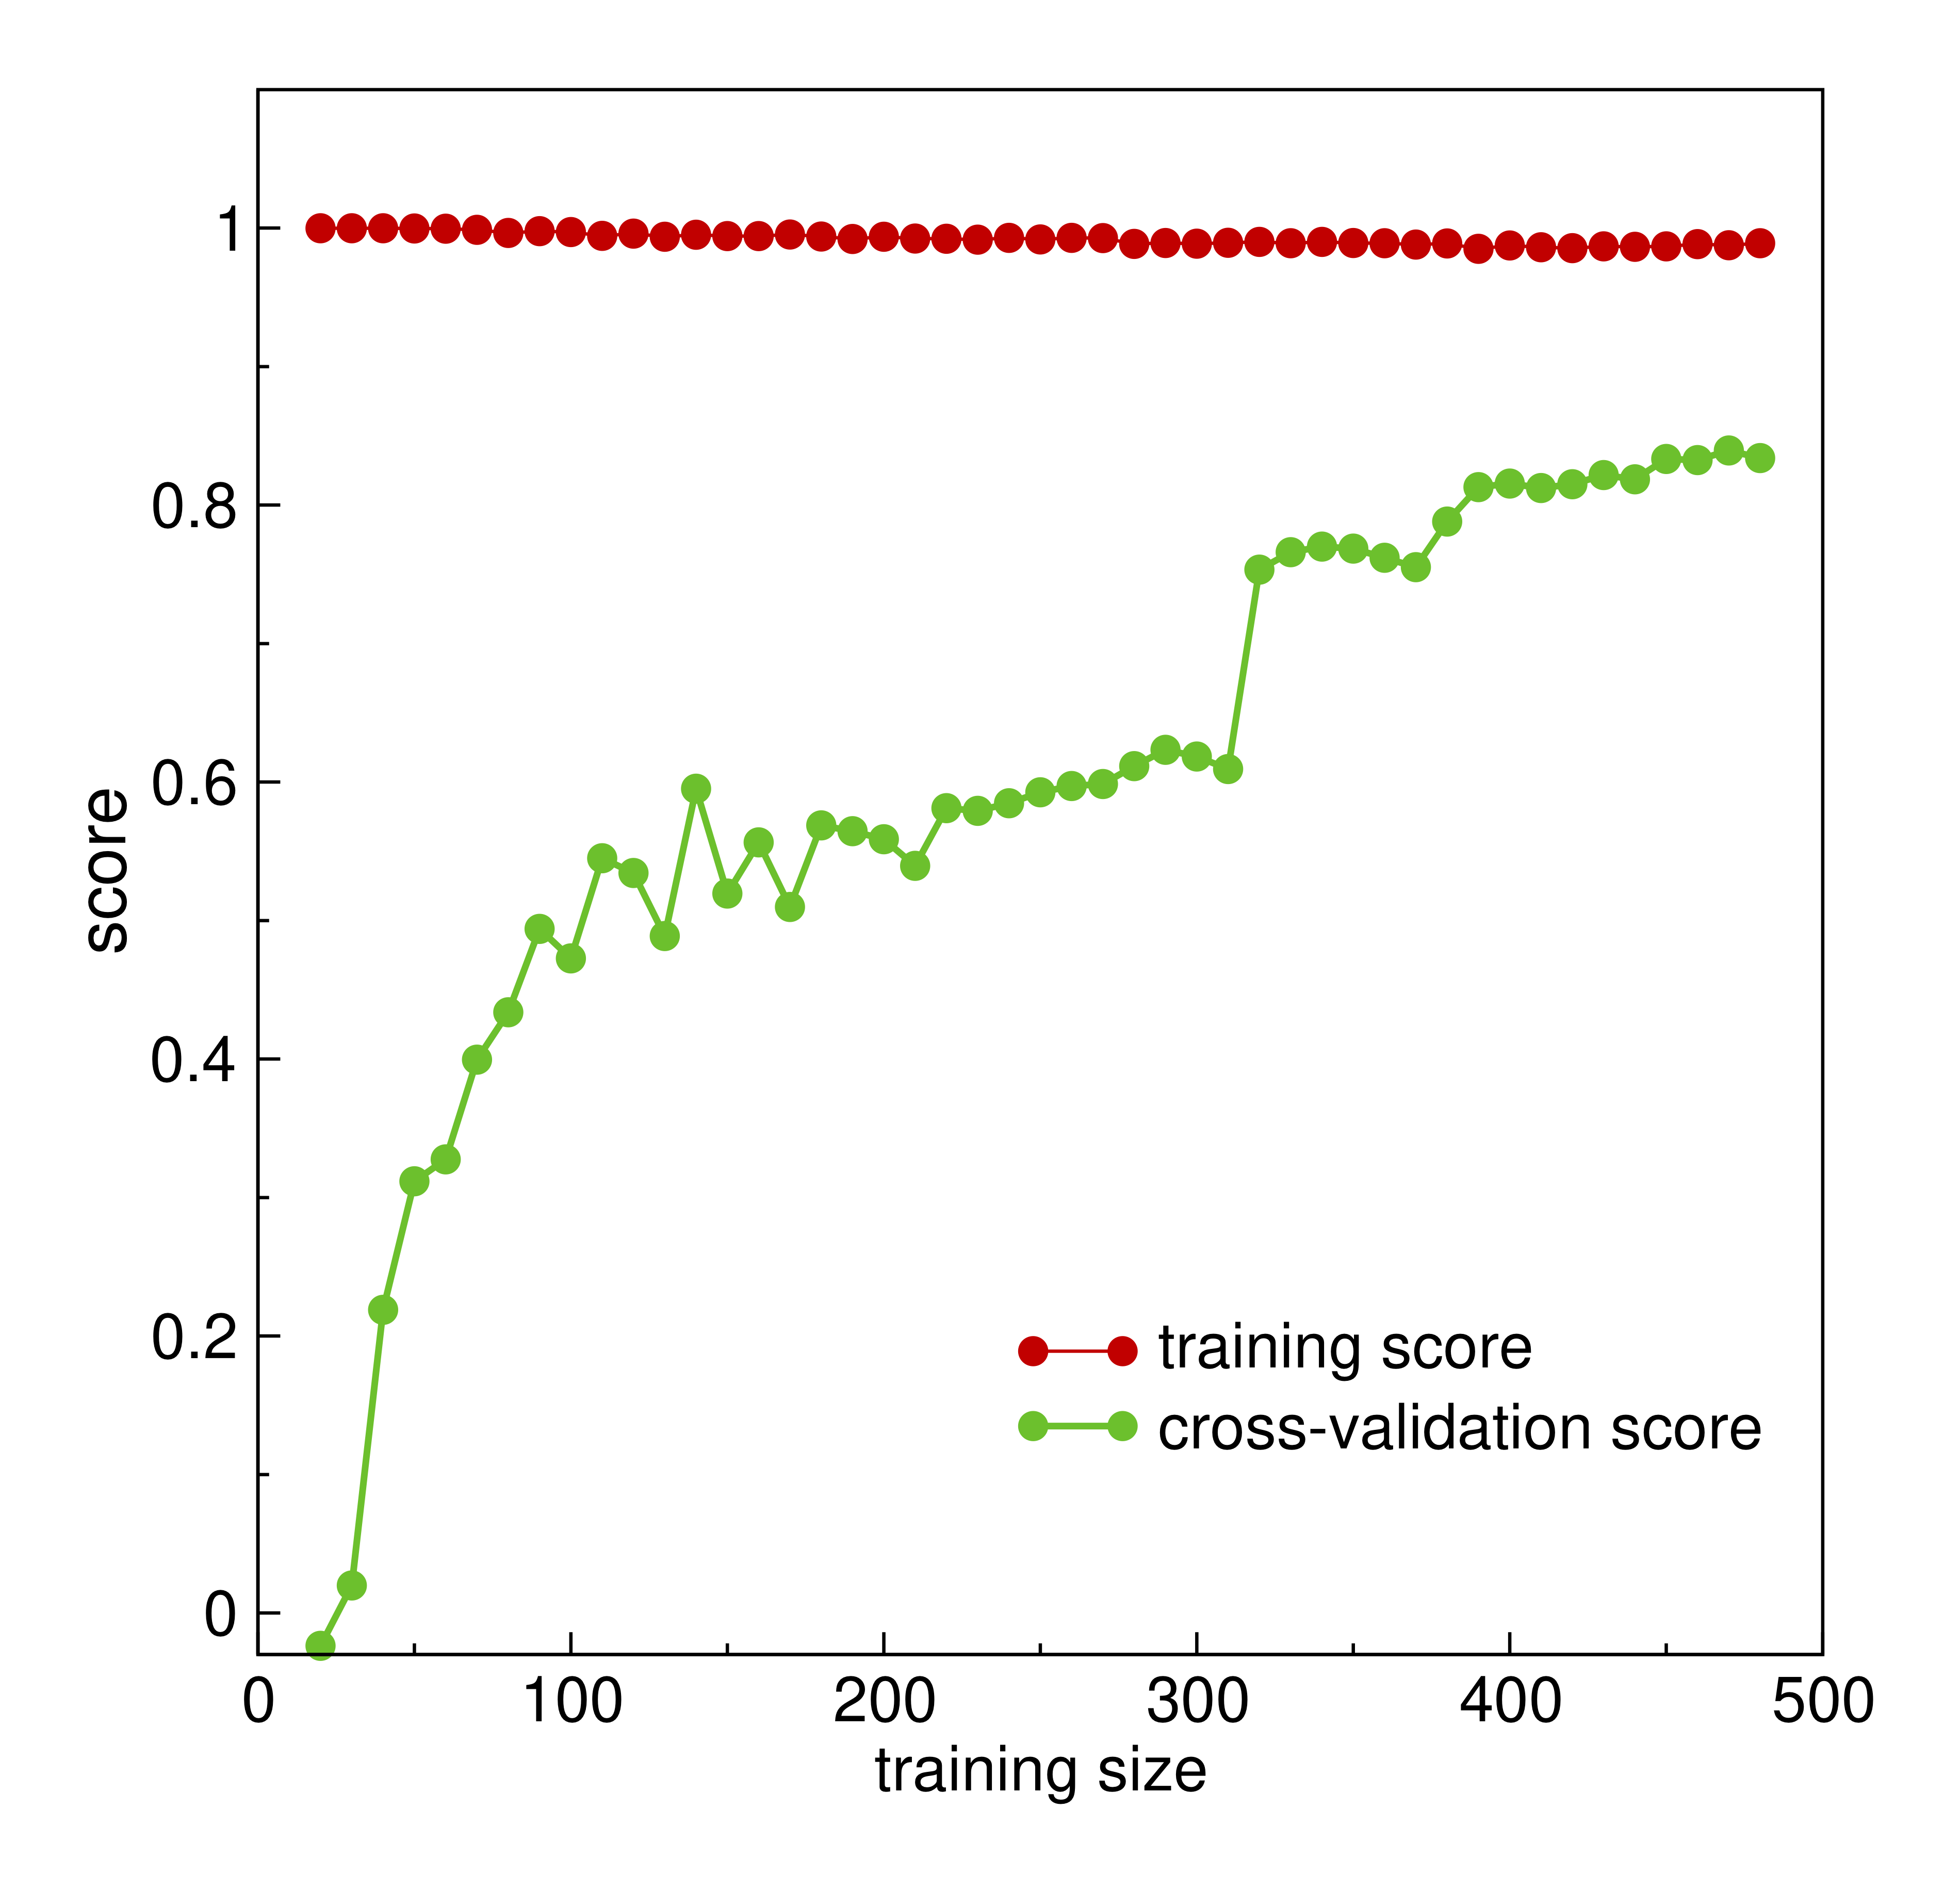
\includegraphics[width=0.95\linewidth]{figures/learning_curve.png}
  \caption{Learning curve of predicting thermal conductivity from chemical composition using XGBoost algorithm.}
  \label{fig:learning_curve}
\end{figure}



%%%%%%%%%%%%%%%%%%%%%%%%%%%%%%%%%%%%
% CONCLUSIONS
%%%%%%%%%%%%%%%%%%%%%%%%%%%%%%%%%%%
\section{conclusions}
We find that machine learning could provide both qualitative and quantitative insights of alloy steel composition-property relationship. Gradient boost-based algorithms outperform the other machine learning algorithms in our benchmark. XGBoost is particularly successful in predicting thermal conductivity using alloy chemical composition, and the performance can be improved by adding more training samples.

\begin{table*}[t]
\begin{ruledtabular}
\caption{Hyper-parameters used in different machine learning algorithms for grid search.\label{tab:hyperparam}}
\centering
\begin{tabular}{ccc}
\sffamily Algorithm & \sffamily Parameter & \sffamily Values \\
\hline
Linear Regression & default & default \\
\hline
Lasso & `alpha' & \{ 1E-4, 0.001, 0.01, 0.1, 1 \}\\
\hline
& `kernel' & \{`linear', `poly', `rbf', `sigmoid' \} \\
Kernel Ridge & `alpha' & \{ 1E-4, 1E-2, 0.1, 1 \} \\
& `gamma' & \{ 0.01, 0.1, 1, 10 \} \\
\hline
Linear SVR & `C' & \{ 1E-6, 1E-4, 0.1, 1 \} \\
& `loss' & \{ `epsilon\_insensitive', `squared\_epsilon\_insensitive'\} \\
\hline
SGD & `alpha' & \{1E-6, 1E-4, 0.01, 1 \} \\
& `penalty' & \{`l2', `l1', `elasticnet'\} \\
\hline
& `activation' & \{`logistic', `tanh', `relu'\} \\
MLP & `solver' & \{`lbfgs', `adam', `sgd'\} \\
& `learning\_rate' & \{`constant', `invscaling', `adaptive'\} \\
\hline
Adaboost & `n\_estimators' & \{10, 100, 1000\} \\
& `learning\_rate' & \{0.01, 0.1, 1, 10\} \\
\hline
& `n\_estimators' & \{10, 100, 1000\} \\
RandForest& `min\_weight\_fraction\_leaf' & \{0.0, 0.25, 0.5\} \\
& `max\_features' & \{`sqrt', `log2', None\} \\
\hline
& `n\_estimators' &  \{10, 100, 1000\}\\
GradBoost & `min\_weight\_fraction\_leaf' &  \{0.0, 0.25, 0.5\}\\
& `max\_feature' &  \{`sqrt', `log2', None\}\\
\hline
& `n\_estimators' &  \{10, 50, 100, 250, 500, 1000\}\\
& `learning\_rate' &  \{1E-4, 0.01, 0.05, 0.1, 0.2\}\\
XGBoost & `gamma' &  \{0, 0.1, 0.2, 0.3, 0.4\}\\
& `max\_depth' &  \{6\}\\
& `subsample' &  \{0.5, 0.75, 1\}\\
\end{tabular}
\end{ruledtabular}
\end{table*}

\clearpage

\section{Supporting information}

\noindent \hypertarget{scrape}{\texttt{\Large{scrape.py}}}
\begin{lstlisting}
  1 #! /home/raymond/.conda/envs/scrape/bin/python
  2 # Author: Raymond Wang <raymondwang@u.northwestern.edu>
  3 # Challenge project from Citrine Informatics
  4 # Functionality: scrape alloy steel data from MatWeb and save to csv files
  5 
  6 from selenium import webdriver
  7 from selenium.webdriver.support.ui import Select
  8 import pandas as pd
  9 import numpy as np
 10 import time
 11 import sys
 12 import os.path
 13 import os
 14 
 15 # navigate to target website
 16 options = webdriver.ChromeOptions()
 17 options.add_argument("headless") # comment this for visualization
 18 driver_path = os.getcwd() + "/chromedriver-linux" # google-chrome driver for Linux
 19 #driver_path = os.getcwd() + "/chromedriver-mac" # google-chrome driver for macOS
 20 driver = webdriver.Chrome(executable_path=driver_path, chrome_options=options)
 21 driver.get("http://www.matweb.com/index.aspx")
 22 
 23 # user login, less likely to be blocked
 24 driver.find_element_by_link_text("LOG IN").click()
 25 time.sleep(2)
 26 username = driver.find_element_by_id("ctl00_ContentMain_txtUserID")
 27 username.send_keys("USERNAME")
 28 passwd =  driver.find_element_by_id("ctl00_ContentMain_txtPassword")
 29 passwd.send_keys("PASSWD")
 30 time.sleep(0.5)
 31 driver.find_element_by_xpath("//input[@src='/images/buttons/btnLogin.gif']").click()
 32 time.sleep(3)
 33 
 34 # Alloy composition
 35 driver.find_element_by_link_text("Alloy Composition").click()
 36 
 37 # unfold "Ferrous Metal"
 38 driver.find_element_by_id("ctl00_ContentMain_ucMatGroupTree_LODCS1_msTreeViewn1").click()
 39 time.sleep(2)
 40 
 41 # choose "Alloy Steel"
 42 driver.find_element_by_id("ctl00_ContentMain_ucMatGroupTree_LODCS1_msTreeViewt6").click()
 43 time.sleep(2)
 44 
 45 # choose composition1: Mn
 46 select_fe = Select(driver.find_element_by_id(
 47     "ctl00_ContentMain_ucPropertyDropdown1_drpPropertyList"))
 48 select_fe.select_by_visible_text("Manganese, Mn")
 49 driver.find_element_by_id(
 50     "ctl00_ContentMain_ucPropertyEdit1_txtpMin").send_keys("0.0")
 51 time.sleep(2)
\end{lstlisting}
\clearpage
\begin{lstlisting}
 52 
 53 # choose composition2: Cr
 54 select_cr = Select(driver.find_element_by_id(
 55     "ctl00_ContentMain_ucPropertyDropdown2_drpPropertyList"))
 56 select_cr.select_by_visible_text("Chromium, Cr")
 57 driver.find_element_by_id("ctl00_ContentMain_ucPropertyEdit2_txtpMin").send_keys("0.0")
 58 time.sleep(2)
 59 
 60 # choose composition3: Ni
 61 select_ni = Select(driver.find_element_by_id(
 62     "ctl00_ContentMain_ucPropertyDropdown3_drpPropertyList"))
 63 select_ni.select_by_visible_text("Nickel, Ni")
 64 driver.find_element_by_id("ctl00_ContentMain_ucPropertyEdit3_txtpMin").send_keys("0.0")
 65 time.sleep(2)
 66 
 67 # lauch searching process
 68 driver.find_element_by_id("ctl00_ContentMain_btnSubmit").click()
 69 time.sleep(3)
 70 
 71 # show 200 per page
 72 instance_per_page = 200
 73 Select(driver.find_element_by_id("ctl00_ContentMain_UcSearchResults1_drpPageSize1"))
 74     .select_by_visible_text(str(instance_per_page))
 75 time.sleep(3)
 76 
 77 # loop over 5 pages of results to collect data
 78 npages = 5
 79 for ipage in range(npages):
 80     print("currently on page " + str(ipage+1))
 81     sys.stdout.flush()
 82 
 83     # save name of datasets to a list before processing,
 84     # may not be ideal design but avoids stale element problems
 85     name_list = []
 86     for item in driver.find_elements_by_xpath(
 87         "//td[@style='width:auto; font-weight:bold;']"):
 88         name_list.append(item.text)
 89 
 90     for name in name_list:
 91         # preprocessing
 92         fname = name.replace(" ", "_")
 93         fname = fname.replace("/", "_")
 94         fname = fname.replace(",", "")
 95         # in case length of file name exceeds Linux limit (255B)
 96         if len(fname) > 240: fname = fname[:240]+"..."
 97         pathname = "data_raw/" + fname + ".csv"
\end{lstlisting}
\clearpage
\begin{lstlisting}
 98         if os.path.isfile(pathname):
 99             if os.stat(pathname).st_size == 0: # in case last written unsuccessful
101                 os.remove(pathname)
102             else:
104                 continue
105       
106         sys.stdout.flush()
107 
108         # open file
109         f = open("data_raw/" + fname + ".csv", 'w')
110 
111         # navigate into each alloy page
112         driver.find_element_by_link_text(name).click()
113         time.sleep(5)
114         table = driver.find_element_by_xpath("//table[@class='tabledataformat']")
115         attrib = []
116         for row in table.find_elements_by_xpath("//tr[@class='altrow datarowSeparator']"):
117             attrib.append([d.text for d in row.find_elements_by_css_selector('td')])
118             time.sleep(0.5)
119         for row in table.find_elements_by_xpath("//tr[@class=' datarowSeparator']"):
120             attrib.append([d.text for d in row.find_elements_by_css_selector('td')])
121             time.sleep(0.5)
122         attrib = np.array(attrib)
123 
124         # write to file
125         df = pd.DataFrame(data=attrib[:, 1:], columns=['Metric', 'English', 'Comments'],
126             index=attrib[:, 0] )
127         df.to_csv(f)
128         f.close()
129         driver.back()
130         time.sleep(5)
131 
132     # navigate to the next page
133     driver.find_element_by_id("ctl00_ContentMain_UcSearchResults1_lnkNextPage").click()
134     time.sleep(5)
135 
136 # quit chrome driver
137 driver.quit()
\end{lstlisting}

\clearpage
\noindent \hypertarget{pprocess}{\texttt{\Large{post\_processing.py}}\label{code:postprocess}}
\begin{lstlisting}
  1 import os
  2 
  3 ddir = "./data_raw/"
  4 # modify filenames
  5 for filename in os.listdir(ddir):
  6     newname = filename
  7     for ch in filename:
  8         if (ch in ['.', '_', '-']) or (47 < ord(ch) 58) or (64 < ord(ch) < 91)
  		 or (96 < ord(ch) < 123): continue
  9         else: newname = newname.replace(ch, "")
 10     newname = newname.replace("__", "_")
 11     os.rename(ddir+filename, ddir+newname)
 12 
 13 # fix unwanted new lines and non-utf-8 encodings
 14 for filename in os.listdir(ddir):
 15     content = open(ddir+filename, errors='ignore').read()
 16     new_cont = content.replace("\n@", " @")
 17     f = open(ddir+filename, 'w')
 18     f.write(new_cont)
 19     f.close()
 20 import os
 21 
 22 # fix feature name problems
 23 str1 = "string_to_be_replaced"
 24 str2 = "new_string"
 25 for filename in os.listdir(ddir):
 26     content = open(ddir+filename, errors='ignore').read()
 27     new_cont = content.replace(str1, str2)
 28     f = open(ddir+filename, 'w')
 29     f.write(new_cont)
 30     f.close()
\end{lstlisting}


\clearpage
\noindent \hypertarget{featurize}{\texttt{\Large{featurize.py}}}
\begin{lstlisting}
  1 from collections import defaultdict
  2 import pandas as pd
  3 import os
  4 
  5 ## select features and convert from strings to floating point numbers
  6 
  7 features_dict = defaultdict(int)
  8 
  9 ddir = "../scrape_data/data_raw/"
 10 for filename in os.listdir(ddir):
 11     data = pd.read_csv(ddir+filename, header=0, index_col=0)
 12     for ind in data.index:
 13         features_dict[ind] += 1
 14 
 15 print(' These are the potential features:')
 16 for ii in sorted(features_dict.items(), key=lambda tup: tup[-1], reverse=True):
 17     if (ii[-1] > 100) and (ii[0] is not ' '):
 18         print(ii)
 19 print('')
 20 
 21 elem_list = ['Iron, Fe', 'Carbon, C', 'Sulfur, S', 'Silicon, Si', 
 22              'Phosphorous, P', 'Manganese, Mn', 'Chromium, Cr', 
 23              'Nickel, Ni', 'Molybdenum, Mo', 'Copper, Cu']
 24 
 25 prop_list = ['Density', 'Hardness, Vickers', 'Thermal Conductivity',
 26              'Specific Heat Capacity', 'CTE, linear', 'Electrical Resistivity',
 27              'Elongation at Break', 'Bulk Modulus', 'Modulus of Elasticity',
 28              'Shear Modulus', 'Poissons Ratio', 'Tensile Strength, Yield',
 29              'Tensile Strength, Ultimate']
 30 
 31 feature_list = elem_list + prop_list
 32 nfeature = len(feature_list)
 33 
 34 # collect features from files
 35 data_all_string = []
 36 for filename in os.listdir(ddir):
 37     instance = ['0%']*len(elem_list) + ['NA']*len(prop_list) # initialize instance row
 38     data = pd.read_csv(ddir+filename, header=0, index_col=0)
 39     for ii in range(nfeature): 
 40         if feature_list[ii] in data.index:
 41             instance[ii] = data.loc[feature_list[ii], 'Metric']
 42             # get rid of some unexpected '\n' in dataset
 43             if '\n' in instance[ii]: instance[ii] = instance[ii].replace('\n', ' ')
 44     if instance[0] is not 0: data_all_string.append(instance) # steel only
 45 
 46 # convert to DataFrame and save to file
 47 data_all_string = pd.DataFrame(data_all_string, index=None, columns=feature_list)
 48 data_all_string.to_csv(path_or_buf="../data/data_all_string.csv", sep=';', index=False)
 49 
\end{lstlisting}
\clearpage
\begin{lstlisting}
 50 # define util function
 51 def extract_float(string):
 52     if string is 'NA': return string # do not process non-available data
 53     num1 = ''
 54     num2 = ''
 55     curr = 0
 56     while not string[curr].isdigit(): # locate the first digit
 57         curr += 1
 58     # process the first float
 59     assert(string[curr].isdigit())
 60     while string[curr].isdigit():
 61         num1 += string[curr]
 62         curr += 1
 63         if curr == len(string): return float(num1)
 64     if string[curr] is '.':
 65         num1 += '.'
 66         curr += 1
 67         while string[curr].isdigit():
 68             num1 += string[curr]
 69             curr += 1
 70             if curr == len(string): return float(num1)
 71     # check if there is a second
 72     while string[curr].isspace():
 73         curr += 1
 74     if string[curr] is not '-':
 75         return float(num1)
 76     else: # process the second float
 77         curr += 1
 78     while string[curr].isspace():
 79         curr += 1
 80     assert(string[curr].isdigit())
 81     while string[curr].isdigit():
 82         num2 += string[curr]
 83         curr += 1
 84         if curr == len(string): return (float(num1) + float(num2)) / 2.0
 85     if string[curr] is '.':
 86         num2 += '.'
 87         curr += 1
 88         while string[curr].isdigit():
 89             num2 += string[curr]
 90             curr += 1
 91             if curr == len(string): return (float(num1) + float(num2)) / 2.0
 92     return (float(num1) + float(num2)) / 2.0
\end{lstlisting}
\clearpage
\begin{lstlisting}
 93 
 94 
 95 # convert string to float
 96 data_all_float = pd.DataFrame(data=data_all_string, copy=True)
 97 for ii in range(data_all_float.shape[0]):
 98     for jj in range(data_all_float.shape[1]):
 99         data_all_float.iloc[ii, jj] = extract_float(data_all_float.iloc[ii, jj])
100 
101 # drop instances whose Fe weight is less than 50%
102 drop_list = []
103 for ii in data_all_float.index:
104     if data_all_float.loc[ii, 'Iron, Fe'] < 80.:
105         drop_list.append(ii)
106 data_all_float = data_all_float.drop(drop_list)
107 
108 print('Shape of data: ', data_all_float.shape)
109 data_all_float.to_csv("../data/data_all_float.csv", sep=';', index=False)
\end{lstlisting}


\clearpage
\noindent \hypertarget{correlation}{\texttt{\Large{correlation.py}}}\
\begin{lstlisting}
  1 import pandas as pd
  2 import seaborn as sns; sns.set()
  3 import matplotlib.pyplot as plt
  4 import numpy as np
  5 import math
  6 import os
  7 
  8 data = pd.read_csv("../data/data_all_float.csv", header=0, index_col=None, sep=';')
  9 
 10 # drop instances with NaN
 11 drop_list = []
 12 for idx in data.index:
 13     if True in [math.isnan(x) for x in data.loc[idx].values]:
 14         drop_list.append(idx)
 15 data = data.drop(drop_list)
 16 print('The shape of data: ', data.shape)
 17 
 18 corr = data.corr()
 19 
 20 fig = plt.figure(num=None, figsize=(40, 40), dpi=80, facecolor='w', edgecolor='w')
 21 colormap = sns.diverging_palette(220, 10, as_cmap=True)
 22 mask = np.zeros_like(corr)
 23 mask[np.triu_indices_from(mask)] = True
 24 ylabel = list(corr.columns)
 25 ylabel[0] = ''
 26 ax = sns.heatmap(corr, cmap=colormap, mask=mask, annot=True, fmt=".2f",
 27 xticklabels=corr.columns[:-1], yticklabels=ylabel)
 28 plt.title(label="Correlation Heatmap of All Features", loc='center', fontdict={
 29          'fontname':'DejaVu Sans', 'size':'24', 'color':'black', 'weight':'bold',
 30          'verticalalignment':'bottom'})
 31 ax.tick_params(axis='x', rotation=60, labelsize=10)
 32 ax.tick_params(axis='y', labelsize=13)
 33 plt.show()
 34 fig.savefig("heatmap_mask.png", dpi=200)
\end{lstlisting}

\clearpage
\noindent \hypertarget{ml}{\texttt{\Large{benchmark.py}}}
\begin{lstlisting}
  1 import numpy as np
  2 import pandas as pd
  3 import sys
  4 import operator
  5 import math
  6 
  7 import xgboost
  8 from sklearn.preprocessing import StandardScaler
  9 from sklearn.model_selection import GridSearchCV, train_test_split
 10 from sklearn.metrics import *
 11 
 12 import warnings
 13 warnings.filterwarnings("ignore", category=DeprecationWarning)
 14 warnings.filterwarnings("ignore", category=UserWarning)
 15 warnings.filterwarnings("ignore", category=FutureWarning)
 16 
 17 
 18 data = pd.read_csv("../data/data_all_float.csv", header=0, index_col=None, sep=';')
 19 
 20 # drop 'CTE, linear' for more instances to study
 21 drop_feature = ['Density', 'CTE, linear']
 22 for ifeature in drop_feature:
 23     data = data.drop(labels=ifeature, axis=1)
 24 
 25 # drop instances with NaN
 26 drop_instance = []
 27 for idx in data.index:
 28     if True in [math.isnan(x) for x in data.loc[idx, data.columns.values]]:
 29         drop_instance.append(idx)
 30 data = data.drop(drop_instance)
 31 
 32 print('Shape of dataset:')
 33 print(data.shape)
 34 
 35 hyper_params = [{
 36     'n_estimators' : (10, 50, 100, 250, 500, 1000,),
 37     'learning_rate' : (0.0001,0.01, 0.05, 0.1, 0.2,),
 38     'gamma' : (0,0.1,0.2,0.3,0.4,),
 39     'max_depth' : (6,),
 40     'subsample' : (0.5, 0.75, 1,),
 41 }]
 42 
 43 stdscale = StandardScaler()
 44 
 45 properties = [ 'Thermal Conductivity', 'Specific Heat Capacity', 'Hardness, Vickers',
 46                'Electrical Resistivity', 'Elongation at Break', 'Bulk Modulus',
 47                'Modulus of Elasticity', 'Shear Modulus', 'Poissons Ratio',
 48                'Tensile Strength, Yield', 'Tensile Strength, Ultimate']
 49 
\end{lstlisting}
\clearpage
\begin{lstlisting}
 50 for target in properties:
 51     print('current target: ', target)
 52     
 53     X = data.drop(target, axis=1).values
 54     y = data[target].values
 55 
 56     # standardize features
 57     X = stdscale.fit_transform(X)
 58     y = stdscale.fit_transform(y.reshape(-1, 1))
 59 
 60     X_train, X_test, y_train, y_test = train_test_split(X, y, train_size=0.75,
 61    		 test_size=0.25, random_state=0)
 62 
 63     regressor = xgboost.XGBRegressor()
 64 
 65     grid_clf = GridSearchCV(regressor, cv=5, param_grid=hyper_params,
 66              verbose=1, n_jobs=8, scoring='r2')
 67 
 68     grid_clf.fit(X_train, y_train.ravel())
 69 
 70     train_score_mse = mean_squared_error(stdscale.inverse_transform(y_train),
 71              stdscale.inverse_transform(grid_clf.predict(X_train)))
 72     test_score_mse = mean_squared_error(stdscale.inverse_transform(y_test),
 73      	 stdscale.inverse_transform(grid_clf.predict(X_test)))
 74 
 75     sorted_grid_params = sorted(grid_clf.best_params_.items(), key=operator.itemgetter(0))
 76 
 77     # print results
 78     out_txt = '\t'.join(['algorithm: ', str(sorted_grid_params).replace('\n', ','),
 79                str(train_score_mse), str(test_score_mse)])
 80 
 81     print(out_txt)
 82     print("")
 83     sys.stdout.flush()
\end{lstlisting}


\end{document}



